Functional analysis defines how \abbr{EWAS} performs its mission from initial observation to warning delivery and long-term system improvement. It describes the main operational flows between the \abbr{GEO} and \abbr{LEO} satellite layers, the ground segment, and the national authority users. The purpose of this section is to clarify the sequence of functions required to detect a potential missile launch, process and validate the event, estimate the threat trajectory and impact area, disseminate an alert, and maintain the system during routine and crisis operations.

\begin{figure}[htbp]
    \centering
    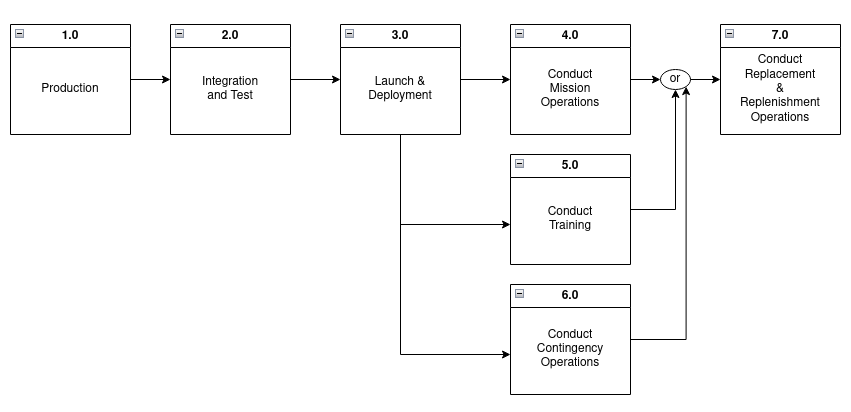
\includegraphics[width=0.9\textwidth]{Figures/general_flow_2.png}
    \caption{Top Level Flow}
    \label{fig:general-flow}
\end{figure}




\subsection{Primary Threat Detection and Warning Flow}
The primary responsibility of the \abbr{EWAS} mission is to detect missile threats worldwide, determine whether they could affect the Baltic region, and generate dedicated alerts for emergency authorities. This mission is conducted in accordance with the functional flow shown in Figure~\ref{fig:mission-operation-flow}.

The combined constellation of six \abbr{GEO} satellites and 72 high-inclination \abbr{LEO} satellites is responsible for detecting unusual thermal bursts. \abbr{GEO} satellites provide persistent wide-area observation where viewing geometry is favorable, while \abbr{LEO} satellites provide high-elevation coverage at high latitudes. The detecting satellite conducts denoising to rule out solar bursts, Earth background noise, and other non-threat thermal signatures.

In case of an unusual burst detection, the burst coordinates are sent to the two \abbr{LEO} satellites closest to the detected location. The two \abbr{LEO} satellites track the potential missile from different observation angles and calculate a preliminary stereoscopic trajectory. They then transmit the encrypted telemetry and preliminary trajectory estimate to the Ground Segment.

Finally, the Ground Segment decrypts the received telemetry data and confirms its integrity. It then fuses the observations to calculate the definitive trajectory and estimated impact zone. The system generates an alert, which is then sent to the appropriate national authority body.


\begin{figure}[htbp]
    \centering
    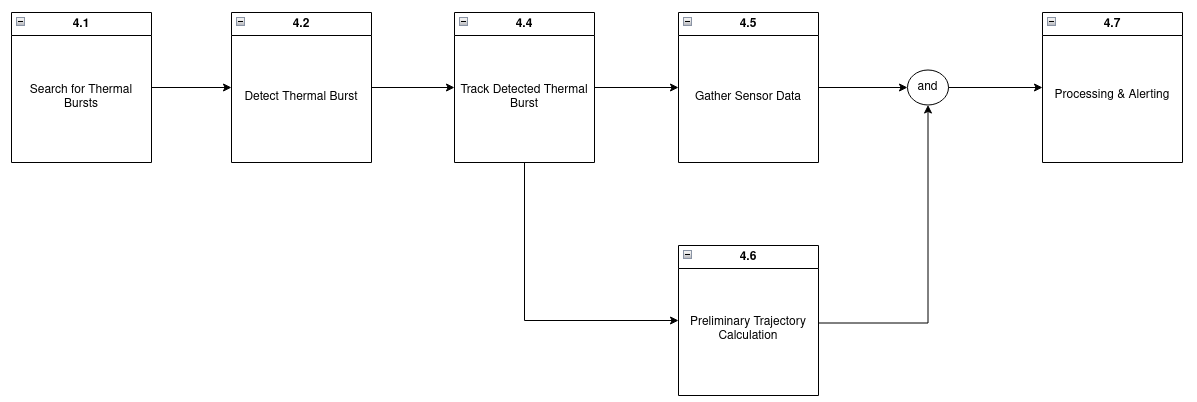
\includegraphics[width=0.9\textwidth]{Figures/warning_flow_2.png}
    \caption{Second Level Flow}
    \label{fig:mission-operation-flow}
\end{figure}


\subsection{Data Management and Continuous Improvement Flow}

This flow operates asynchronously to the primary warning flow, fulfilling the mission's objective to use historical data for system refinement and national resilience.

\begin{itemize}
    \item Archive all raw sensor readings, onboard processing logs, telemetry records, and final generated warning outputs in encrypted system storage.
    \item Retrieve historical event data for authorized post-event technical analysis, lessons-learned review, and missile characterization.
    \item Use archived data to refine detection, classification, denoising, tracking, and impact-area estimation algorithms.
    \item Reduce false alarm rates by comparing confirmed missile events with non-threat thermal signatures such as solar bursts and Earth background noise.
    \item Prepare validated software and algorithm updates for the space segment and ground processing center.
    \item Securely uplink approved updates to satellites and deploy them to the ground segment during planned operation and maintenance windows.
    \item Share sanitized historical event data with partner governments and international crisis-response mechanisms when authorized.
\end{itemize}

\subsection{System Maintenance and Support Flow}

This background operational loop ensures that \abbr{EWAS} maintains high availability, reliable coverage, and stable performance during both routine operation and crisis conditions.

\begin{itemize}
    \item Continuously monitor satellite health and status telemetry from the space segment.
    \item Verify communication links between \abbr{GEO} satellites, \abbr{LEO} satellites, ground stations, and national authority interfaces.
    \item Perform attitude and orbit control to maintain required satellite pointing, orbital positioning, and coverage of the monitored region.
    \item Regulate spacecraft power and thermal conditions using the Electrical Power System (\abbr{EPS}) and Thermal Control System (\abbr{TCS}).
    \item Detect subsystem anomalies and initiate fault-management procedures when degraded performance is observed.
    \item Maintain ground segment hardware, processing infrastructure, databases, and operator consoles.
    \item Apply tested software patches and configuration updates to preserve redundant and uninterrupted operations.
\end{itemize}